\documentclass{report}

\usepackage{amsmath}
\usepackage{physics}
\usepackage{mhchem}
\usepackage[labelfont=bf]{caption}
\usepackage{graphicx}
\usepackage{comment}
\usepackage{color, soul}    % for text highlighting

\usepackage[style=phys]{biblatex}       % citations!
\addbibresource{main.bib}

% Defines the subfigure environment
\usepackage{subcaption}

% Puts the abstract on the title page
\usepackage{titling}
\newsavebox{\abstractbox}
\renewenvironment{abstract}
 {%
  \global\setbox\abstractbox=\vtop\bgroup
  \begin{center}\bfseries\abstractname\end{center}%
 }
 {\par\egroup}
\renewcommand{\maketitlehookd}{%
  \par\vfil
  \box\abstractbox
}

% Changes the formatting of the chapter numbers
\usepackage{titlesec}
\titleformat{\chapter}
  {\normalfont\LARGE\bfseries}{\thechapter}{1em}{}
\titlespacing*{\chapter}{0pt}{3.5ex plus 1ex minus .2ex}{2.3ex plus .2ex}


% TITLE DATA
\title{Development of a Visible Photoluminescence Microspectrometer}
\author{Zach Colbert}
\date{Spring 2019}


% For comments, notes, todos, etc.
\newcommand{\printnote}[2]{\hl{[\textbf{#1: #2}]}}
\newcommand{\todo}[1]{\printnote{TODO}{#1}}
\newcommand{\note}[1]{\printnote{NOTE}{#1}}


\begin{document}
  % TITLE PAGE
  % \begin{titlingpage}
    % \begin{abstract}
      % This is the abstract. It comes later.
    % \end{abstract}
    % \maketitle
  % \end{titlingpage}

  \begin{titlepage}
    \begin{center}
        \vspace*{1cm}
  
        \textbf{Development of a Visible Photoluminescence Microspectrometer}
  
        \vspace{1.5cm}
  
        by \\
        \textbf{Zachary Colbert}
  
        \vspace{5cm}
  
        A thesis advised by Matt W. Graham \\
        submitted to \\
        Oregon State University

        \vspace{1.5cm}

        in partial fulfillment of \\
        the requirements for the degree of \\
        Baccalaureate of Science in Physics
  
        \vfill
  
        Presented X June 2019 \\
        Commencement June 2020
  
    \end{center}
  \end{titlepage}

  \thispagestyle{plain}
\begin{center}
    \Large \textbf{Development of a Visible-NIR Photoluminescence Microspectrometer}
 
    \vspace{0.4cm}
    by \\
    \textbf{Zachary Colbert}
 
    \vspace{0.9cm}
    \textbf{Abstract}
\end{center}

This is the abstract. It's coming soon.

  \tableofcontents
  \listoffigures


  \chapter{Introduction}
  % \section{The Need for a Simpler Spectrometer (Motivation)}
The Graham Micro-Femto Energetics ($\mu fE$) group at Oregon State University uses advanced optoelectronic methods to characterize materials, especially thin-layer materials and micron-scale semiconducting devices.

The group's workhorse when it comes to PL measurements is a Horiba \textbf{Something?} fluorimeter, coupled to a \textbf{Something?} microscope. The system uses a \textbf{Specs?} lamp and double-monochromator to illuminate a wide field with a tunable wavelength.

The wide field illumination is really nice for imaging, but makes it hard to isolate emissions from small spatial domains.

Something about visible and NIR detectors. NIR detector requires liquid nitrogen.

Something about the system takes a long time to warmup before the light source is stable.

Something about training time and the learning curve for using the device. Software is kinda complicated. Takes a really long time to take a measurement.

To address this, I build my system to be user friendly and easy to learn.

Naturally, my system has fewer applications. It only measures emission (not excitation), and modifications to the system are a little more complicated. But it's great for taking initial measurements of a sample. If more complicated stuff needs to be done, use the fluorimeter.

Also, my system has much better spatial resolution because it uses a laser source. This makes it less good for imaging, but that can be overcome.

  \chapter{Background}
  \subsection{Optoelectronic Materials}

Optoelectronic materials convert light to electric energy and/or electric energy to light. The study of these materials goes back as far as the early 1900s, but accelerates rapidly in the 1960s with the advent of the light emitting diode and semiconductor laser \cite{sweeney_optoelectronic_2017}. Optoelectronic devices are ubiquitous; they have enabled the rapid growth of information technologies around the world, and are fundamental in modern telecommunication and internet infrastructure. Modern optronics research explores new materials that can be used to create faster, more efficient, and smaller optoelectronic devices.

\subsubsection{Organic Photovoltaic: ADT}

Organic optoelectronic materials are not a new discovery, but have become increasingly popular in recent decades as methods for creating them have advanced \cite{ostroverkhova_organic_2016}. The Ostroverkhova group at Oregon State University have studied several organic photovoltaics (OPVs) including functionalized derivatives of pentacene, benzothiophene, and anthradithiophene (ADT) \cite{shepherd_optical_2010}\cite{e._b._shepherd_effect_2011}\cite{platt_optical_2009}. A drop-cast sample of fluorinated ADT with triethylsilyethynyl (TES) functional group, provided by the Ostroverkhova group, is used for demonstration of the new microspectrometer device in Chapter \ref{chap:results}.

\begin{figure}[H]
    \centering
    \includegraphics{img/adt-tes-f.png}
    \caption[Molecular diagram of ADT TES-F.]{Molecular diagram of fluorinated anthradithiophene (ADT) with triethylsilyethynyl (TES) side group \cite{shepherd_optical_2010}. A drop-cast sample of this molecule was provided by the Ostroverkhova group at Oregon State University, and used for demonstration of our microspectrometer instrument following a study by Lam \cite{lam_polarization_2018}.}
    \label{fig:adt-diagram}
\end{figure}

\subsubsection{Quantum Dots: \ce{CdSe}}

\subsection{Photoluminescence}
Photoluminescence (PL) is a mechanism by which materials absorb and emit photons. The process can be described with respect to electronic transitions within an atom or molecule.

The absorptive transition occurs first, when a photon interacts with a molecule and is absorbed. The photon's energy must be approximately equal to the bandgap of the absorbing molecule to satisfy the energy transitions allowed by quantum mechanics. When that condition is met, the photon's energy raises an electron to an excited state, where it stays for a short time.

Some number of vibronic transitions occur as the electron loses energy to radiation and vibration. \todo{How do we measure these transitions, or their lifetimes?}

Finally, the radiative transition occurs when the electron decays back to a ground state. During the radiative transition, a photon is emitted at the bandgap energy as the electron moves from the lowest vibronic state in the conduction band to the highest vibronic state in the valence band. \todo{This needs some work.}

\subsection{PL as a Characteristic Measurement}
\todo{Why is PL a useful measurement in solid state? In biological sciences? In general?}


  \chapter{Methods}
  \subsection{Design}

\subsubsection{Microscope}

The starting point of the project was an Olympus BX60M fluorescence microscope. The BX60M is built for reflection microscopy, and includes a housing for brightfield and darkfield mirrors. For the new instrument, we added a mirror cube housing between the brightfield/darkfield mirror housing and the observation tube. This additional component housed a dichroic mirror, which enabled us to couple an external light source into the instrument and filter that light out of the path through the observation tube.

\subsubsection{Laser Excitation}
The BX60M is equipped with a xenon arc lamp, which is used for general observations under white light illumination. In order to measure photoluminescence, we require the use of a (mostly) monochromatic light source which is energetic enough to excite electrons in the sample.

\begin{figure}[H]
    \centering
    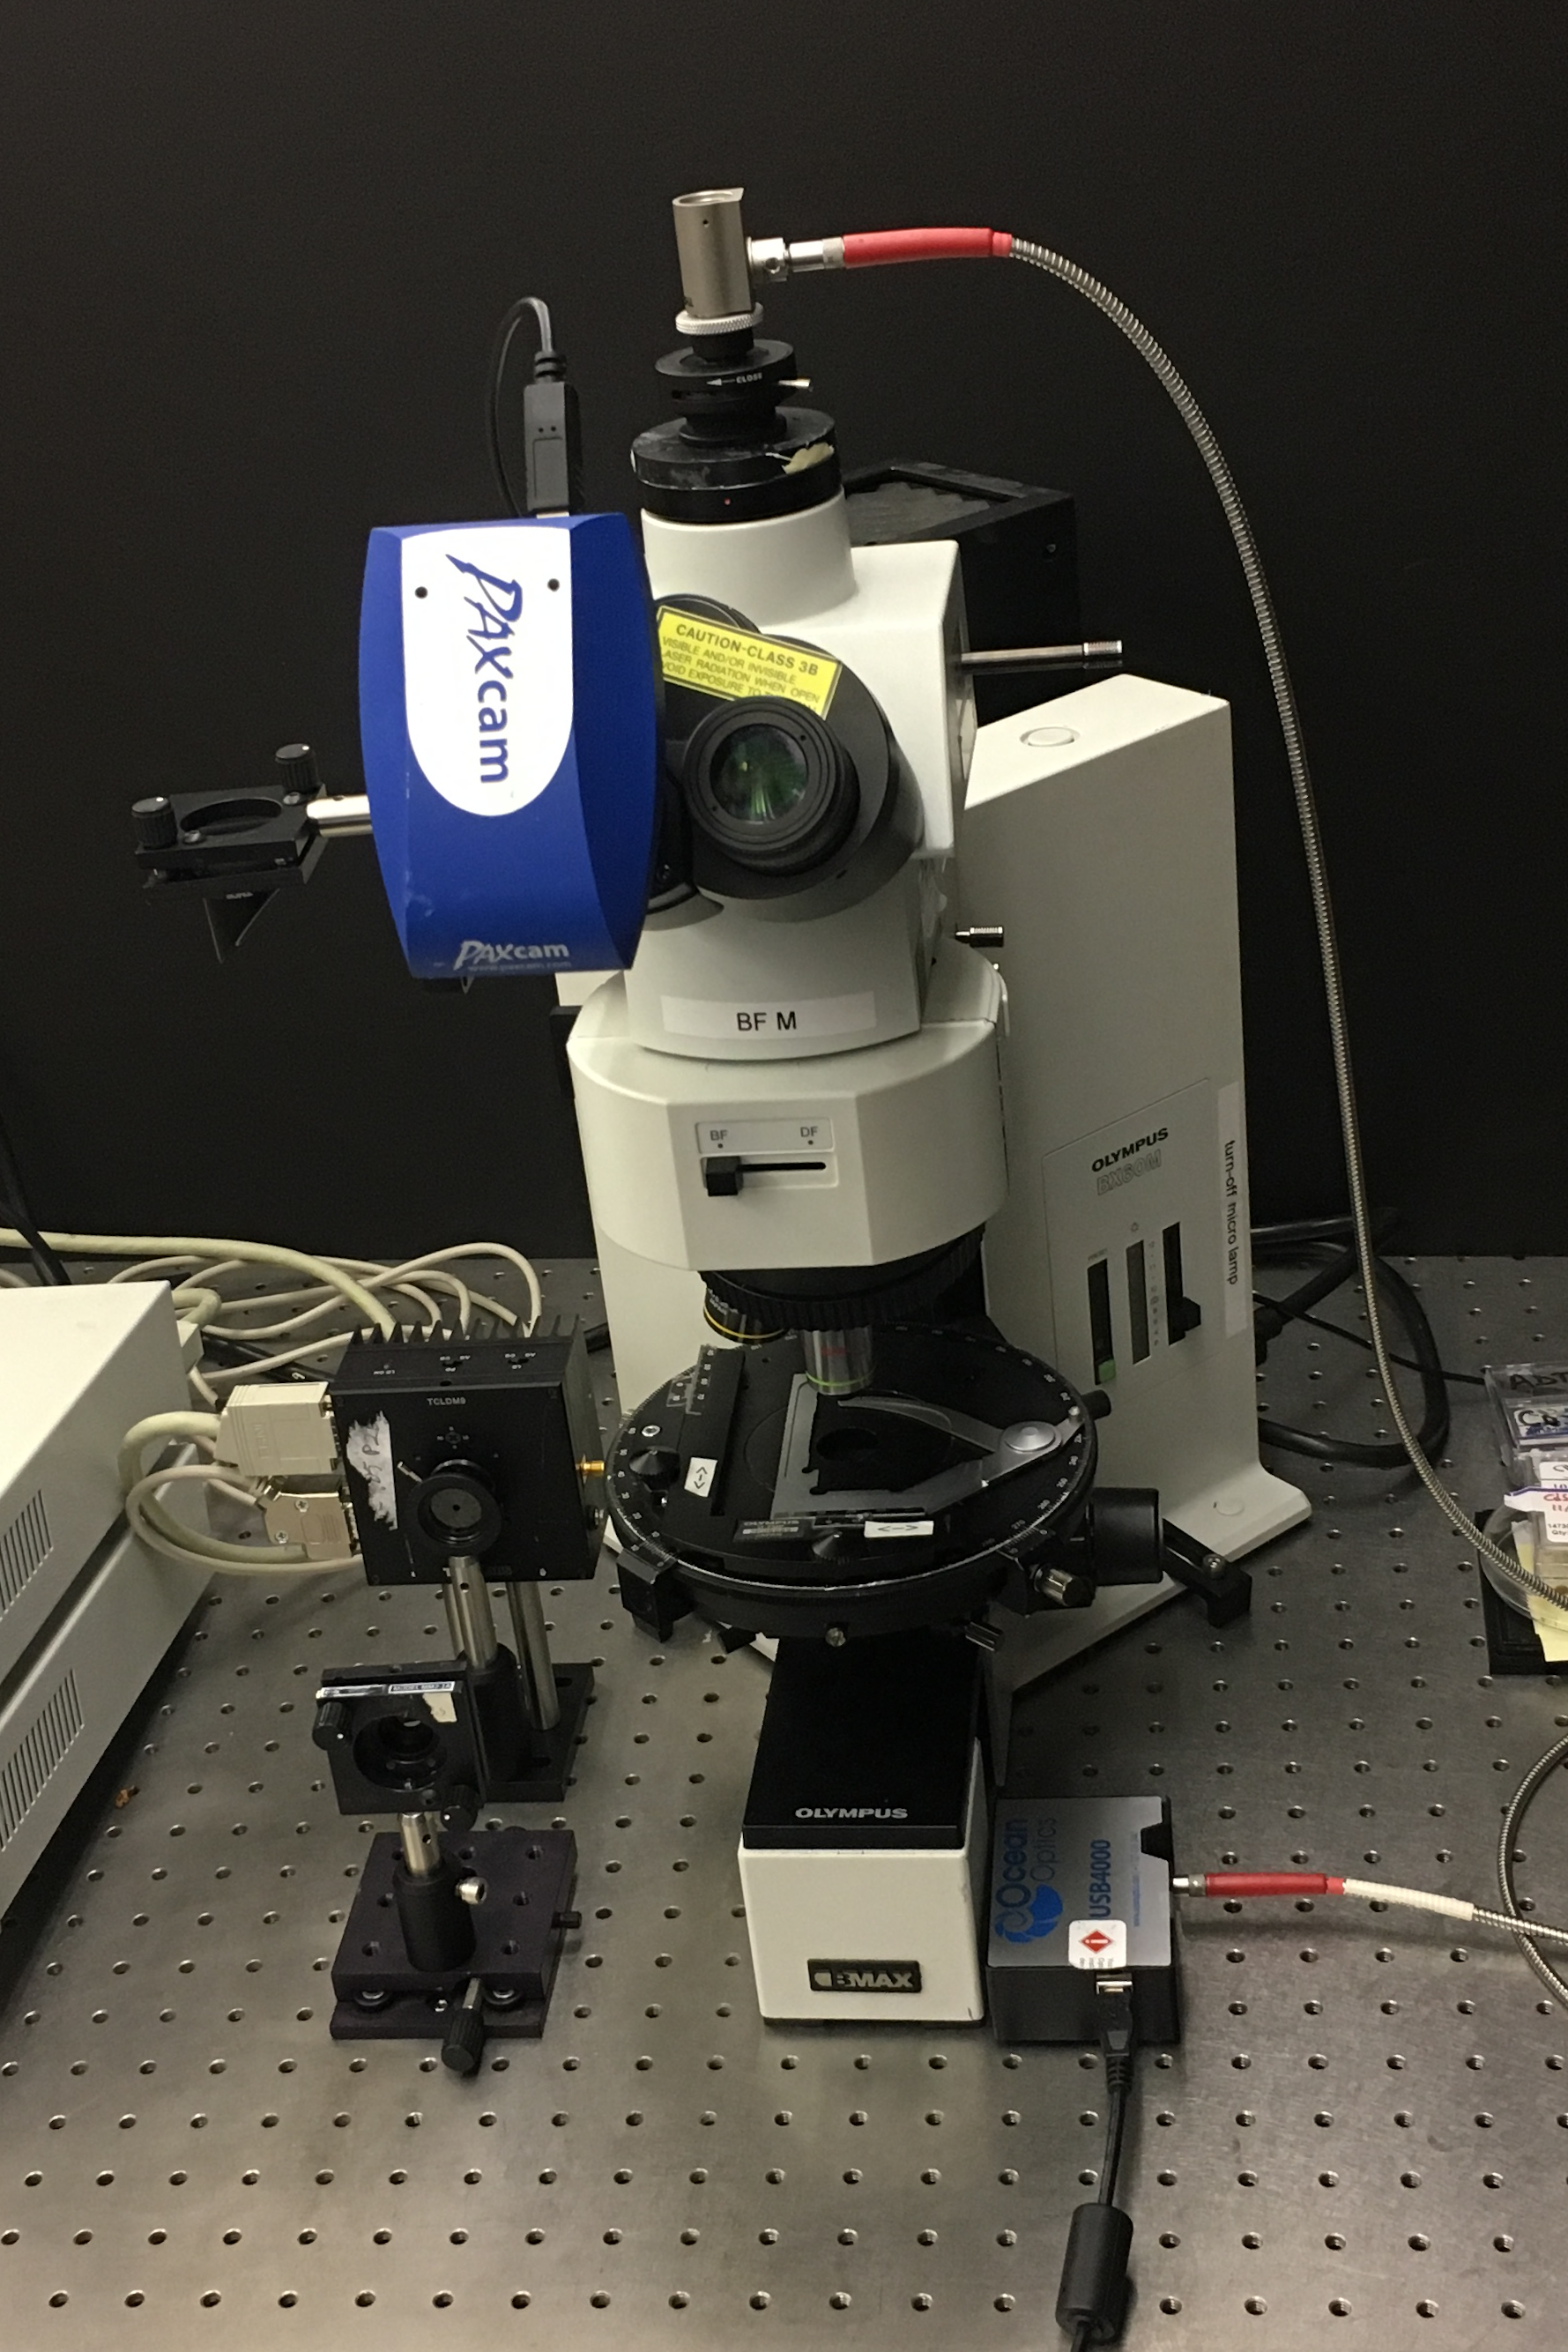
\includegraphics[width=0.5\textwidth]{img/microscope.png}
    \caption[Front view of microspectrometer instrument.]{Front view of microspectrometer instrument (laser controllers not pictured) built around Olympus BX60M fluorescence microscope. The laser diode mount and mirrors are shown on the left. Digital camera for sample imaging is mounted to the microscope eyepiece. We have mounted a collimating mirror to the observation tube (at the top of the microscope), which collects emissions and transmits them into a USB spectrometer via optical fiber.}
    \label{img:microscope}
\end{figure}

Our instrument uses a diode laser as its light source. Specifically, we used a ThorLabs L405P20 laser diode (405 nm), TCLDM9 thermoelectrically-cooled mount, LDC 202 laser diode controller, and TED 200 temperature controller. To couple the laser and microscope, we used a set of two mirrors in a vertical beam fold configuration. This enabled precise alignment of the laser to the optical axis of the microscope, maximizing transmission of excitation light through the objective lens and onto the sample stage.

\begin{figure}[h]
    \centering
    \includegraphics[width=.75\textwidth]{img/optical-diagram.png}
    \caption{Schematic diagram of the microspectrometer instrument.}
    \label{img:optical-diagram}
\end{figure}

The laser diode housing and first mirror were mounted to an optical table. The laser starts parallel to the surface of the table and the first mirror directs the beam upward. The second mirror in the beam fold was mounted to the end of a tube that extends out the side of the mirror cube housing. This mirror directs the vertical beam horizontally into the mirror. It seems preferable to mount both mirrors to the optical table for stability, but we were successful with this method by mounting the microscope to the table so that it and the second mirror did not move relative to the laser beam during normal operation.

\begin{figure}[H]
    \centering
    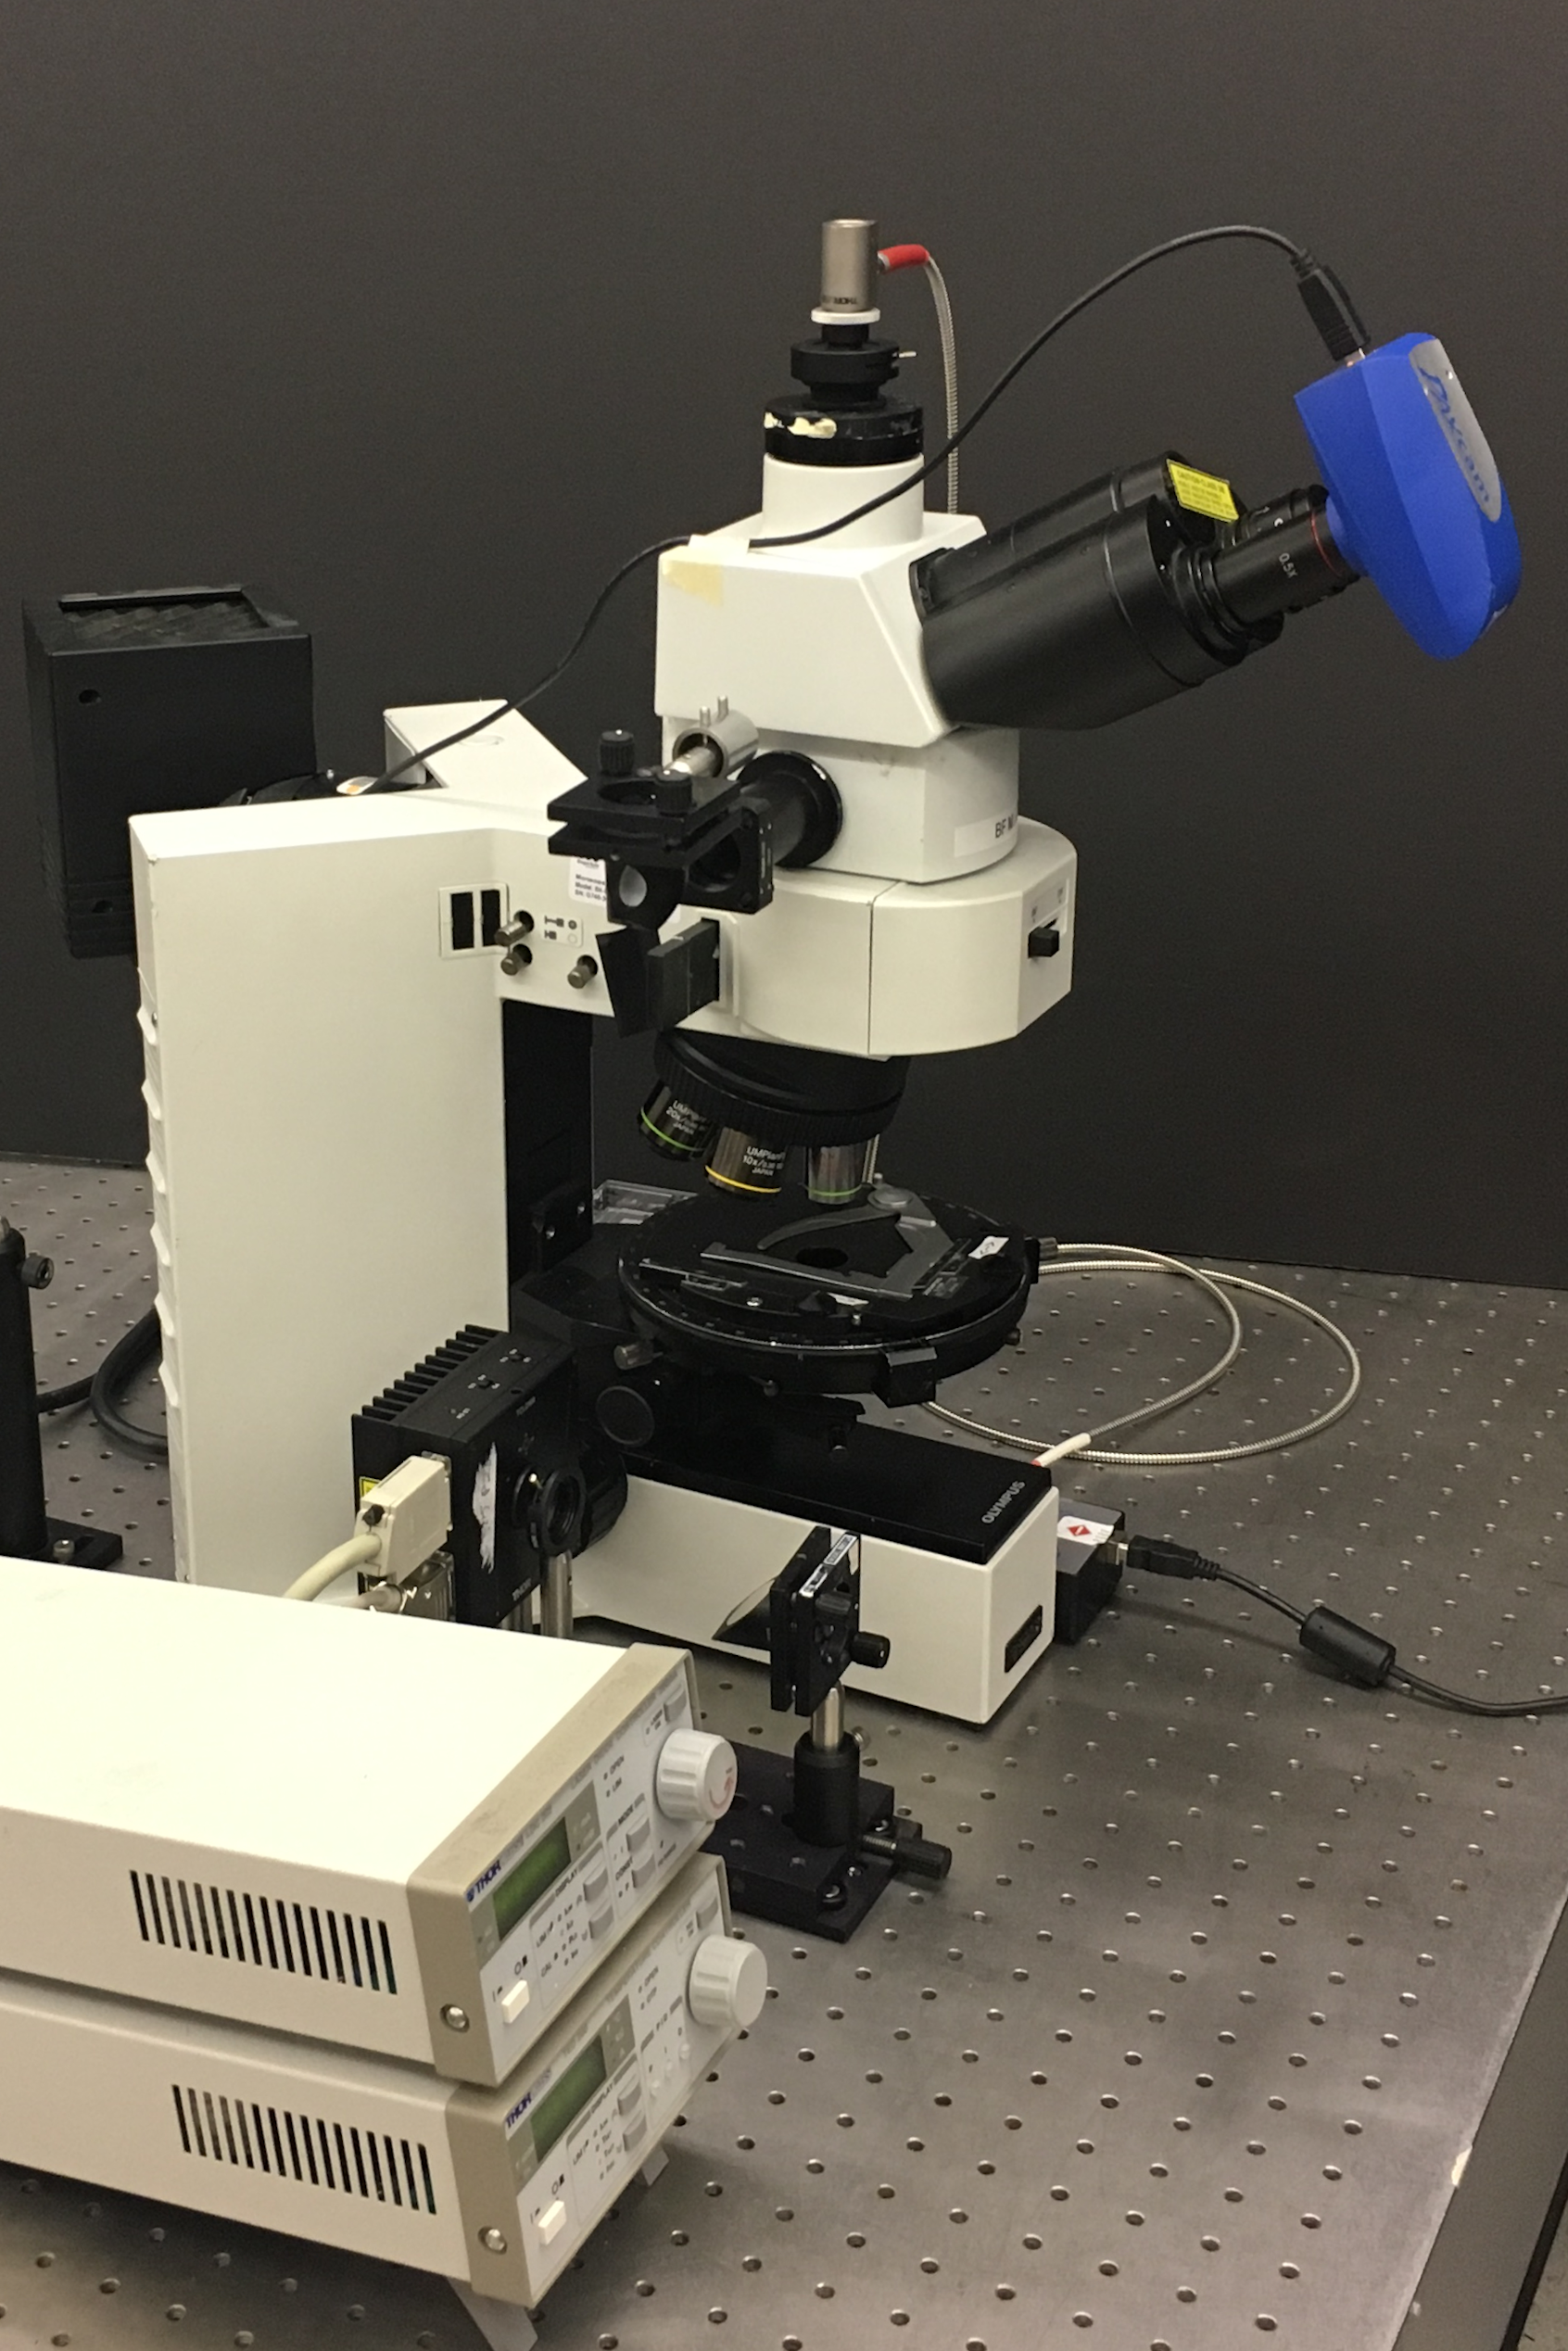
\includegraphics[width=0.5\textwidth]{img/microscope-side.png}
    \caption[Side view of microspectrometer instrument.]{Side view of microspectrometer instrument. Laser controllers are shown in the foreground. Between the controllers and the microscope, two flat mirrors and a dichroic mirror (not visible here) couple the laser light into the microscope's optical path.}
    \label{img:microscope-side}
\end{figure}

It was not feasible to align the laser diode housing and mirror cube housing in the plane of the table due to limited space on the optical table. To overcome this, our beam fold configuration also turns the beam 90 degrees in the plane of the table. The configuration we used has the laser beam initially pointed in the direction of the operator, then directed upward by the first mirror, then directed into the side of the mirror cube housing. While in operation, but particularly during laser alignment, precautions must be taken to protect the operator's eyes from direct exposure to the laser beam. The optical power of the laser is low enough that laser safety glasses (with high optical density near 405 nm) are sufficient, but beam blocks on the table may also be desireable in some cases.

We used a longpass dichroic mirror with a cutoff wavelength slightly higher than the excitation wavelength at 405 nm, causing nearly all of the excitation light to be reflected in the direction of the sample. A longpass mirror with cutoff wavelength slightly higher than the excitation wavelength is ideal beacuse it will pass most of the light emitted by the sample, as we expect fluorescence to nearly always have a longer wavelength than the exciting photons.

% Because fluorescence will nearly always have a longer wavelength than the exciting photons, we expect the mirror to pass most of the light emitted by the sample and block any reflected excitation light.

The observation tube on the Olympus BX60M is at the top of the microscope's optical path; the operator can toggle between using the observation tube or binocular optic. To collect and measure the spectrum of fluorescent emissions, we fixed a collimating adapter to the observation tube. This allowed us to collect emissions and transmit them via optical fiber to our spectromter.

We used an Ocean Optics (now Ocean Insight) USB2000 miniature spectrometer to measure the spectra shown in Chapter \ref{chap:results}. The USB2000 is sensitive to light between about 350 nm and 1000 nm, so in this case we are only able to measure fluorescent emissions in the visible spectrum and a small part of the near-infrared spectrum. This detector can easily be exchanged for one with a different range as required for future projects.

The USB spectrometer is connected to a nearby desktop computer, with Ocean Optics software installed for measuring spectra.

\begin{figure}[H]
    \centering
    \includegraphics[width=0.75\textwidth]{img/objective-sample.JPG}
    \caption[Sample on stage under laser illumination.]{A sample of CdSe quantum dots under laser illumination at 405 nm. Some of the violet laser light is reflected by the sample, but is difficult to distinguish from the sample's intense green emission.}
    \label{img:objective-sample}
\end{figure}

We were able to fix a digital camera to the binocular optic for simple imaging of samples with adapters on hand. The camera is connected via USB to a desktop computer with software for capturing images. Example images are shown in Figures \ref{img:tesf} and \ref{img:qd}.


\subsection{Laser Alignment}
We align the laser to the microscope's optical axis by iteratively adjusting the two flat mirrors that direct the beam into the side of the microscope. First, we adjust the position of the beam as it enters the mirror cube housing by moving the first mirror. A reticle made of photoluminescent laser viewing material was a particularly useful target when fixed to the opening on the side of the mirror cube housing. 

We then adjust the second mirror in the beam fold to change the angle at which the beam is incident on the dichroic mirror. This translates the beam across the back of the microscope nosepiece, where our target is the optical axis of the objective lens. In place of a lens, we fix an iris diaphragm to the nosepiece. We adjust the second mirror to position the laser in the center of the mostly-closed iris, which marks the location of the optical axis of a lens. This process is repeated until the laser spot is centered on both targets.



  \chapter{Results and Discussion}
  
In this chapter we demonstrate the use of the new microspectrometer instrument by measuring photoluminescence in samples of two materials, introduced in Chapter \ref{chap:intro-optomats}. Samples of the anthradithiophene derivative ADT-TES-F and of cadmium selenide quantum dots were both drop-cast from solution on glass slides. Both samples were excited at 405 nm, with our detector measuring emissions between approximately 450 nm and 1000 nm.

For each sample we were able to measure PL in approximately the same regions of interest with both the Horiba Fluorolog-3 and our new instrument. Figures \ref{fig:pl-adt-tesf} and \ref{fig:pl-adt-qd} compare the resulting spectra measured by each device. 

We also demonstrate the use of our instrument for imaging. Figures \ref{img:tesf} and \ref{img:qd} show images of the region of interest used for PL measurements of each sample. 

\begin{figure}[H]
    \centering
    \begin{subfigure}[b]{0.45\textwidth}
        \includegraphics[width=\textwidth]{./img/tesf-white-illum.png}
        % \caption{TESF region of interest under white light.}
        \caption{}
        \label{img:tesf-white}
    \end{subfigure}
    \hfill
    \begin{subfigure}[b]{0.45\textwidth}
        \includegraphics[width=\textwidth]{./img/tesf-laser-illum.png}
        % \caption{TESF region of interest under excitation light.}
        \caption{}
        \label{img:tesf-laser}
    \end{subfigure}
    \caption[Images of ADT TES-F sample.]{Images of ADT TES-F sample under white light (\ref{img:tesf-white}) and under laser excitation light (\ref{img:tesf-laser}). Reflected excitation light was optically filtered out of Figure \ref{img:tesf-laser} using a dichroic mirror and colored glass longpass filter. Photoluminescence spectra of this region are shown in Figure \ref{fig:pl-adt-tesf}.}
    \label{img:tesf}
\end{figure}

\begin{figure}[H]
    \centering
    \includegraphics[width=0.8\textwidth]{./img/tesf-2.png}%\llap{\raisebox{4cm}{\includegraphics[width=2cm]{img/tesf-white-illum.png}}}
    % \includegraphics[width=.2\textwidth]{./img/tesf-white-illum.png}
    % \includegraphics[width=.2\textwidth]{./img/tesf-laser-illum.png}
    \caption[PL emission spectrum of ADT TES-F, excited at 405nm.]{PL emission spectrum of ADT TES-F, excited at 405 nm.}
    \label{fig:pl-adt-tesf}
\end{figure}

The results from the microspectrometer show an emission maximum at 630 nm for the ADT TES-F sample; a less intense local maximum is also shown at about 600 nm. The spectrum measured with the Fluorolog has similar features to that of the microspectrometer, but is not precisely the same. The peak appears narrower overall in the Fluorolog data than in the microspectrometer data. The lower-wavelength side of the peak begins to rise at a higher wavelength in the Fluorolog data, and the emission maximum is red-shifted by about 4 nm. The local maximum at 600 nm is much less prominent in the Fluorolog data than in the microspectrometer data.

The microspectrometer data shows emission peaks similar to the ones reported by Shepherd \emph{et al.}, who used a similar drop cast sample and the same model Ocean Optics spectrometer \cite{e._b._shepherd_effect_2011}. Unlike Shepherd, we were not able to calibrate our detector with a reliable instrument; this could be a cause for the slight shift between peaks in the Fluorolog data as compared to our microspectrometer data.

Crystal aggregates and orientation with respect to the polarization of the excitation light have been shown to affect the emission spectra in ADT derivatives \cite{lam_polarization_2018}. As shown in Figure \ref{img:tesf}, we were able to excite what appears to be a single crystal domain --- assuming that this domain has few defects and a relatively uniform stacking structure, we expect it to fluoresce with a distinct spectrum. The Fluorolog excites a much wider area of the sample, which may include many crystal domains, defects, and slightly different stacking structures. Thus, it is conceivable that the resulting fluorescence spectrum is an aggregate of several slightly different spectra.

\begin{figure}[H]
    \centering
    \begin{subfigure}[b]{0.45\textwidth}
        \includegraphics[width=\textwidth]{./img/qd-white-illum.png}
        \caption{}
        \label{img:qd-white}
    \end{subfigure}
    \hfill
    \begin{subfigure}[b]{0.45\textwidth}
        \includegraphics[width=\textwidth]{./img/qd-laser-illum.png}
        \caption{}
        \label{img:qd-laser}
    \end{subfigure}
    \caption[Images of CdSe quantum dot sample.]{Images of CdSe quantum dot sample under white light (\ref{img:qd-white}) and under laser excitation light (\ref{img:qd-laser}). Reflected excitation light was optically filtered out of Figure \ref{img:qd-laser} with a dichroic mirror and colored glass longpass filter. Photoluminescence spectra of this sample are shown in Figure \ref{fig:pl-adt-qd}.}
    \label{img:qd}
\end{figure}

\begin{figure}[H]
    \centering
    \includegraphics[width=0.8\textwidth]{./img/qd-2.png}
    % \includegraphics[width=4cm]{./img/qd-white-illum.png}
    % \includegraphics[width=4cm]{./img/qd-laser-illum.png}
    \caption{PL emission spectrum of a cluster of CdSe quantum dots, excited at 405 nm.}
    \label{fig:pl-adt-qd}
\end{figure}

The microspectrometer data shows an emission maximum at 572 nm for our sample of CdSe quantum dots. Peaks in both the Fluorolog and microspectrometer data are well-aligned, though there is a very slight blue-shift in the higher-wavelength leg of the peak of the Fluorolog data. 

The peak at 572 nm is also reported by Empedocles \emph{et al.} in their paper, "Photoluminescence Spectroscopy of Single CdSe Nanocrystallite Quantum Dots" \cite{empedocles_photoluminescence_1996}. They report a much narrower peak than we found (13 meV FWHM to our 110 meV), but measure PL at a very high excitation intensity. We are unable to thoroughly compare our results to those published by Empedocles because we do not have excitation intensity data, but it is possible that excitation intensity affected the width of our emission peak. It is also possible that fundamental differences in our sample and methods resulted in a wider peak --- it is well known that fluorescence in quantum dots varies with their shape and size, and Empedocles used techniques beyond the scope of this project to measure PL of single quantum dots.

Data from the Fluorolog is notably more noisy than data from our microspectrometer. It is possible that this is the result of smoothing by the Ocean Optics spectrometer and its software, though we have found no evidence to support this. It has been suggested that low excitation intensity when using the Fluorolog may result in noisy data, but we are unable to verify this because we do not have excitation intensity data for either of the instruments used in this work \cite{minot-private}. Future work with our microspectrometer instrument should make optical power measurements a high priority.


  % \chapter{Discussion}
  % % Don't use this file. Results and Discussion have been combined into results.tex

  \chapter{Conclusion}
  % \input(chapters/conclusion.tex)

  \chapter*{Acknowledgements}
%   This is a test citation. \cite{edmund_optics_simplifying_nodate}
  % \input(chapters/acknowledgements.tex)

%   \chapter*{References}
  % \input(chapters/references.tex)
  \printbibliography[title=References]


  \appendix
  \chapter{Code}
  % \input(appendix/code)

\end{document}